\documentclass[12pt]{report}
\usepackage[english]{babel}
\usepackage[utf8x]{inputenc}
\usepackage{amsmath}
\usepackage{graphicx}
\usepackage[colorinlistoftodos]{todonotes}
\usepackage{graphicx}
\usepackage{float}
\usepackage{subfigure}
\usepackage{algorithmic}
\usepackage{algorithm}
\usepackage{pdfpages}
\usepackage{color}
\usepackage[toc,page]{appendix}

% % % % % % % % % % % % % % % % % % % % % %
\begin{document}
% % % % % %Front Page % % % % % % % % % % %
\begin{titlepage}
\center

\textsc{\large Seminar Report On}\\[1.0cm] % Name of your university/college
\textsc{\Large BLOCKCHAIN AND ITS APPLICATIONS}\\[1.0cm] % Major heading such as course name
\textsc{\large Submitted in Partial Fulfillment of the Requirements for the award of \\ Bachelor of Technology in \\ Computer Science and Engineering\\ \\ (2015-2019)}\\[0.5cm] 

\begin{figure}[H]
\centering

\includegraphics[width=0.7\textwidth]{logo.png}\\
%\label{logo}
\end{figure}

\vspace{2.0cm}

\begin{minipage}{0.4\textwidth}
\begin{flushleft} \large
\emph{Submitted By:}\\
\hspace{0.3cm}Vimal P Viswan\\
\hspace{0.4cm}Reg No. MUT15CS058\\
\end{flushleft}
\end{minipage}
~~~~~~~~~~~~~~~~~~~~
\begin{minipage}{0.4\textwidth}
\large
\emph{Guide:} \\
\color{white}...\color{black}Mr. Bineeth Kuriakose\\
\color{white}...\color{black}Asst professor\\
\color{white}...\color{black}Department of CSE 
\end{minipage}\\[2cm]

\textbf{Department of Computer Science and Engineering}\\
\textbf{Muthoot Institute of Technology and Science (MITS)} \\
Varikoli P.O, Puthencruz-682308
\end{titlepage}
% % % % % % % % % % % % % % % % % % % % % % % % %
\newpage\begin{titlepage}
\center


\textsc{ \textbf{MUTHOOT INSTITUTE OF TECHNOLOGY \& SCIENCE}}\\
\textsc{\textbf{Varikoli P.O, Puthencruz-682308}}
\vspace{0.7cm}
\begin{figure}[H]
\centering

\includegraphics[width=0.7\textwidth]{logo.png}\\
%\label{logo}
\end{figure}
\vspace{0.2cm}
\textsc{\large \textbf{ DEPARTMENT OF COMPUTER SCIENCE AND ENGINEERING}}\\
\section*{\centering CERTIFICATE}
%\thispagestyle{empty}
\begin{center}
 This is to certify that the seminar report entitled "Title of Seminar" submitted by \textbf{Vimal P Viswan(MUT15CS058)} of Semester VII is  a bonafide account of the work done by him/her under our supervision\\
\end{center}
\vspace{1.6cm}




\noindent Guide \hspace{3.6cm} Coordinator\hfill Head of the Department
\\
\noindent Mr.Bineeth Kuriakose\hspace{0.9cm}Ms Rakhee M \hfill Dr. Anand Hareendran\\
\noindent Asst. Professor\hspace{2.05cm} Asst. Professor\hfill Asso. Professor\\
\noindent Dept. of CSE\hspace{2.4cm} Dept. of CSE\hfill Dept. of CSE
%\noindent\textbox{Left longer sample text\hfill}\textbox{\hfil Center\hfil}\textbox{\hfill Right




\end{titlepage}
\newpage
\pagenumbering{roman}

\section*{\centering Acknowledgements}
\par This seminar is the result of my hard work wherein I have been helped and supported by several persons and institutions directly and indirectly. Now it is the time to acknowledge their contributions. 

\par First of all to the Great Almighty, the author of knowledge and wisdom for his countless love. I respect and thank \textbf{Dr.Chikku Abraham}, Vice Principal of MITS for giving me the opportunity to do this seminar.
With great respect, I express my sincere thanks to our Head of The Department \textbf{Dr. Anand Hareendran} for all the proper guidance and encouragement. I extent my gratitude to the seminar coordinators \textbf{Asst. Prof.Rakhee M}, \textbf{Prof. Dr. Raju.C.K} and \textbf{Asst. Prof. Resmi.N.G} for their timely advice, meticulous scrutiny, scholarly advice and scientific approach that helped to a very great extent throughout the seminar. I would like to sincerely thank my guide \textbf{Asst. Prof. Bineeth Kuriakose}, for his support and valuable guidance.

\par I express my heartfelt veneration to all who had been helpful and inspiring throughout this endeavour.


\null\hfill {Vimal P Viswan}
\newpage

\section*{\centering Abstract}
The seminar topic chosen by me is Blockchain and its Applications.Blockchain is an emerging technology that has got a huge potential applications in the market.It is defined as a growing list of records, called blocks, which are linked using cryptography. Each block contains a cryptographic hash of the previous block, a timestamp, and transaction data. By design, a blockchain is resistant to modification of the data. It is "an open, distributed ledger that can record transactions between two parties efficiently and in a verifiable and permanent way". Once recorded, the data in any given block cannot be altered retroactively without alteration of all subsequent blocks, which requires consensus of the network majority.The major discussions in the following report are an overview of the blockchain technology, the consensus algorithm involved and some relevant application of blockchain in some real time problems.The report also discusses the possible challenges that can occur on using blockchain on several applications.
\newpage


\tableofcontents
\addcontentsline{toc}{chapter}{List of Figures}

\listoffigures
%\addcontentsline{toc}{chapter}{List of Tables}
%\listoftables

% % % % % % % %% % % % % % % % % % % % % % % % % %

\chapter{Introduction}
 \par My main project idea is Blockchain based health record management system named Ayush. After our research works over the idea we came to know that our idea is best suit as a blockchain usecase. Blockchain is a tamper-evident, shared digital ledger that records transactions in a public or private peer-to-peer network. Distributed to all member nodes in the network, the ledger permanently records, in a sequential chain of cryptographic hash-linked blocks, the history of asset exchanges that take place between the peers in the network. Instead of relying on a third party, such as a financial institution, to mediate transactions, member nodes in a blockchain network use a consensus protocol to agree on ledger content, and cryptographic hashes and digital signatures to ensure the integrity of transactions.
 \newline
 \par Consensus ensures that the shared ledgers are exact copies, and lowers the risk of fraudulent transactions, because tampering would have to occur across many places at exactly the same time. Cryptographic hashes, such as the SHA256 computational algorithm, ensure that any alteration to transaction input — even the most minor change — results in a different hash value being computed, which indicates potentially compromised transaction input. Digital signatures ensure that transactions originated from senders (signed with private keys) has safely reached the receivers keeping it's integrity.
 \newline
 \par In the coming chapters we will see in detail the basic structure of blockchain and the technical terms regarding the working of a blockchain network, the various applications present for blockchain in the present scenario, and we will also see the various challenges that blockchain faces.
\pagenumbering{arabic}

\chapter{Blockchain: An Overview}

\section{Background}
\par Blockchain is now recognized as the fifth evolution of computing, the missing trust layer of internet. When an information is added onto the blockchain database it is nearly impossible to remove it or to change it. Before we dive into the detailed concepts within blockchain we must be familiarized with the basic terms related to a blockchain like Distributed Network topology, Decentralization, Distributed Ledger, Anonymity, block structure, Digital Signature, Consensus Algorithms.Lets get into them one by one. 
\section{Distributed Network Topology}
\par A distributed network is a type of computer network that is spread over different networks. This provides a single data communication network, which can be managed jointly or separately by each network. Besides shared communication within the network, a distributed network often also distributes processing.Figure 2.1  below shows both centralized network and a decentralized network.


\par When technology is centralized, it typically means that it is controlled and run by a single company, government, or individual. Decentralized technology on the other hand, is run by a network of participants that no one actor can control or shut down.
\begin{figure}
    \centering
    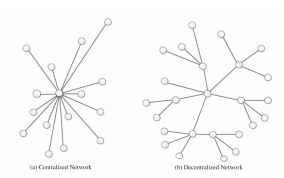
\includegraphics{Blockchain-3.JPG}
    \caption{Distributed Network}
    \label{fig:1}
\end{figure}
\section{Decentralization of Authority}
\par The decentralized nature of blockchain technology means that it doesn’t rely on a central point of control. A lack of a single authority makes the system fairer and considerably more secure. The way in which data is recorded onto a blockchain epitomizes its most revolutionary quality: its value of decentralization. Rather than relying on a central authority to securely transact with other users, blockchain utilizes innovative consensus protocols across a network of nodes, to validate transactions and record data in a manner that is incorruptible. As a blockchain is a ledger of information it is extremely important that the information being stored is honest and accurate.
\section{Distributed Ledger}
\par A distributed ledger is a type of database that is shared, replicated, and synchronized among the members of a decentralized network. The distributed ledger records the transactions, such as the exchange of assets or data, among the participants in the network.
\newline
\par Participants in the network govern and agree by consensus on the updates to the records in the ledger. No central authority or third-party mediator, such as a financial institution or clearinghouse, is involved. Every record in the distributed ledger has a timestamp and unique cryptographic signature, thus making the ledger an auditable, immutable history of all transactions in the network.
\newpage
\chapter{Blockchain Architecture}
\section{A Block}
\par It is a single record inside a list of all records present in a blockchain.A block consists of the block header and the block body as shown in Figure 2.2. It consist of 

\begin{enumerate}
    \item Block version
    \item Timestamp
    \item nBits
    \item Nonce
    \item Parent block hash
\end{enumerate}
\par The block body is composed of a transaction counter and transactions. Asymmetric cryptography and digital signature is used for authentication of transactions. The typical digital signature algorithm used in blockchains is the elliptic curve digital signature algorithm.

\begin{figure}
    \centering
    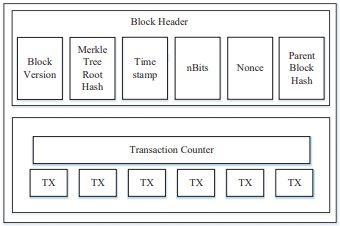
\includegraphics{Blockchain-2.JPG}
    \caption{A Single Block}
    \label{fig:my_label}
\end{figure}
\newpage
\begin{figure}
    \centering
    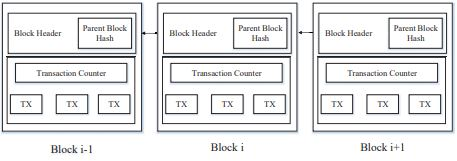
\includegraphics{Blockchain-1.JPG}
    \caption{ An example of blockchain which consists of a continuous
sequence of blocks.}
    \label{fig:my_label}
\end{figure}
\section{Digital Signature}
\par Each user owns a pair of private key and public key.
The private key that shall be kept in confidentiality is used
to sign the transactions. The digital signed transactions are
broadcasted throughout the whole network.First the data is encrypted using senders private key and then at receiver's end it is decrypted using senders public key.
\section{Taxonomy of Blockchain Systems}
\par Current blockchain systems are categorized roughly into
three types: public blockchain, private blockchain and consortium
blockchain.
\par In public blockchain, all records are visible to the public and everyone could take part in the consensus process. Differently, only a group of pre-selected nodes would participate in the consensus process of a consortium
blockchain. As for private blockchain, only those nodes that
come from one specific organization would be allowed to join
the consensus process.A private blockchain is regarded as a centralized network
since it is fully controlled by one organization. The consortium
blockchain constructed by several organizations is partially
decentralized since only a small portion of nodes would be
selected to determine the consensus.
\par The comparison of different types of blockchain with respect to the consensus determination, Read permission, Immutability, Efficiency, Centralized, Consensus process etc are depicted in the figure 2.4.
\begin{figure}
    \centering
    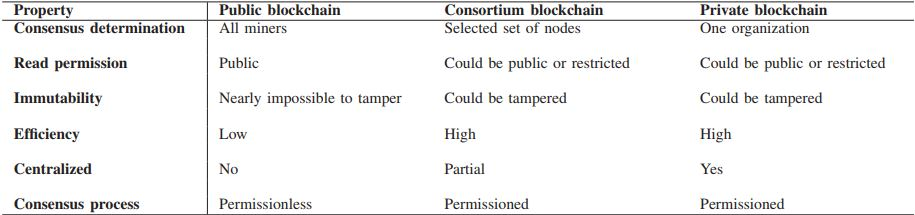
\includegraphics[width=14cm,height=4cm]{Table-1.JPG}
    \caption{Comparison between different types of blockchain}
    \label{fig:my_label}
\end{figure}

\chapter{Consensus Algorithms}
\section{Proof of Work (PoW)}
\par Proof-of-Work, or PoW, is the original consensus algorithm in a Blockchain network. In Blockchain, this algorithm is used to confirm transactions and produce new blocks to the chain. With PoW, miners compete against each other to complete transactions on the network and get rewarded.
\par  In PoW, the block header contains a nonce and miners would change the nonce frequently to get different hash values. The consensus requires that the calculated value must be equal to or smaller than a certain given value. When one node reaches the target value, it would broadcast the block to other nodes and all other nodes must mutually confirm the correctness of the hash value. If the block is validated, other miners would append this new block to their own blockchains.The main disadvantage with this algorithm is that is causes a huge amount of electricity(To run the mining farm) wastage even though it provides more security.
\section{Proof of Stake (PoS)}
\par Proof of Stake is an energy-saving alternative to PoW. Miners in PoS have to prove the ownership of the amount of currency.Proof of Stake (PoS) concept states that a person can mine or validate block transactions according to how many coins he or she holds. This means that the more Bitcoin or altcoin owned by a miner, the more mining power he or she has. In this a validator would be randomly picked who is in charge of ordering the transaction. Thus everyone in the networking is not mining for validation of the transaction but only the validators , which inturn reduces the amount of resources spent.
As less amount of resources are spent on validating the block it is more vulnerable for attacks compared to the Proof of Work algorithm.
\section{Practical Byzantine Fault Tolerance (PBFT)}
\par The PBFT model primarily focuses on providing a practical Byzantine state machine replication that tolerates Byzantine faults (malicious nodes) through an assumption that there are independent node failures and manipulated messages propagated by specific, independent nodes. The algorithm is designed to work in asynchronous systems and is optimized to be high-performance with an impressive overhead runtime and only a slight increase in latency.
\section{Delegated Proof of Stake (DPoS)}
\par Delegated Proof of Stake (DPOS) is the fastest, most efficient, most decentralized, and most flexible consensus model available. DPOS leverages the power of stakeholder approval voting to resolve consensus issues in a fair and democratic way. All network parameters, from fee schedules to block intervals and transaction sizes, can be tuned via elected delegates. Deterministic selection of block producers allows transactions to be confirmed in an average of just 1 second. Perhaps most importantly, the consensus protocol is designed to protect all participants against unwanted regulatory interference.
\section{Ripple Consensus Algorithm}
\par  is a consensus algorithm that utilizes
collectively-trusted subnetworks within the larger network. In
the network, nodes are divided into two types: server for
participating consensus process and client for only transferring
funds. Each server has an Unique Node List (UNL). UNL is
important to the server. When determining whether to put a
transaction into the ledger, the server would query the nodes
in UNL and if the received agreements have reached 80%, the
transaction would be packed into the ledger. For a node, the
ledger will remain correct as long as the percentage of faulty
nodes in UNL is less than 20%.
\section{Tendermint Consensus Algorithm}
\par Tendermint is an easy-to-understand, mostly asynchronous, BFT consensus protocol.Participants in the protocol are called validators; they take turns proposing blocks of transactions and voting on them. Blocks are committed in a chain, with one block at each height. A block may fail to be committed, in which case the protocol moves to the next round, and a new validator gets to propose a block for that height. Two stages of voting are required to successfully commit a block; we call them pre-vote and pre-commit. A block is committed when more than 2/3 of validators pre-commit for the same block in the same round.
\begin{figure}
    \centering
    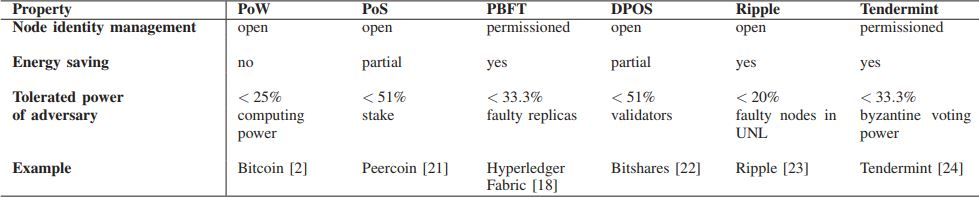
\includegraphics[width=14cm]{Table-2.JPG}
    \caption{Comparison between the various Consensus Algorithm}
    \label{fig:1}
\end{figure}

\chapter{Applications of Blockchain}
\section{Cryptocurrency}
\par Cryptocurrencies have emerged as important financial software systems. They rely on a secure distributed ledger data structure; mining is an integral part of such systems. Mining adds records of past transactions to the distributed ledger known as Blockchain, allowing users to reach secure, robust consensus for each transaction. Mining also introduces wealth in the form of new units of currency. Cryptocurrencies lack a central authority to mediate transactions because they were designed as peer-to-peer systems. They rely on miners to validate transactions. Cryptocurrencies require strong, secure mining algorithms.
\begin{figure}
    \centering
    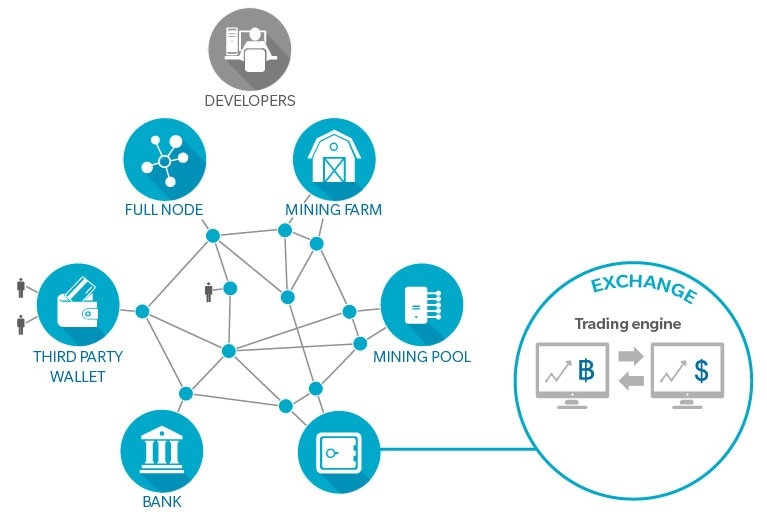
\includegraphics[width=14cm,height=7cm]{cryptocurrency.jpg}
    \caption{Cryptocurrency Network}
    \label{fig:my_label}
\end{figure}
\par In this the private and public keys are kept in wallets. Crypto wallets can be online, offline, software, hardware or even paper. Some can be downloaded for free or are hosted by websites. Others are more expensive.Let's consider the different cryptocurrencies available in market. First of all we have the Bitcoin.
\subsection{Bitcoin}
\par Bitcoin is a digital currency (also called crypto-currency) that is not backed by any country's central bank or government. Bitcoins can be traded for goods or services with vendors who accept Bitcoins as payment.Bitcoin-to-Bitcoin transactions are made by digitally exchanging anonymous, heavily encrypted hash codes across a peer-to-peer (P2P) network. The P2P network monitors and verifies the transfer of Bitcoins between users. Each user's Bitcoins are stored in a program called a digital wallet, which also holds each address the user sends and receives Bitcoins from, as well as a private key known only to the user. 
\section{Healthcare}
\par The impact of blockchain technology can also be
seen in the healthcare industry also. Technologists and healthcare providers
and professionals across the globe view blockchain technology as a crucial
way to implement the sharing of medical records in a secure way to protect
patient’s personal data from outsiders, and give patients more control over
their information.Various blockchain based solutions have been emerged to
enhance current situation of healthcare.
\vspace{10cm}

\begin{figure}
    \centering
    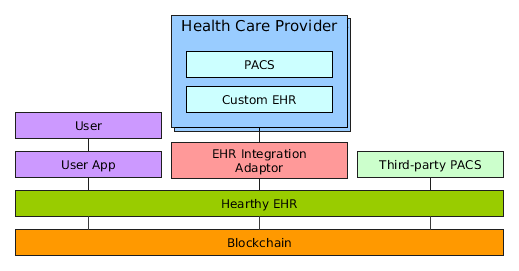
\includegraphics[width=14cm,height=5.5cm]{healthcare.png}
    \caption{Healthcare System Architecture}
    \label{fig:my_label}
\end{figure}
\subsection{MedRec}
\par MedRec uses the blockchain smart contracts to  create a decentralized content-management system for your  healthcare  data, across providers. The MedRec authentication log governs medical  record access, while providing means for auditability and data sharing. A  modular design integrates with providers' existing, local data storage  solutions, enabling interoperability and making our system convenient  and adaptable.
\section{Supply Chain Management}
\par Supply-chain management, also referred to as supply network or logistics network, is a data system of things, goods, and people involved in the process of trading. It is the record of the process involved when the product travels from the place it was made to the person who actually receives it.
\par Recent quality scandals reveal the importance of
quality management from a supply chain perspective.
Although there has been many related studies focusing on
supply chain quality management, the technologies used still
have difficulties in resolving problems arising from the lack of
trust in supply chains. The root reason lies in three challenges
brought to the traditional centralized trust mechanism:
\begin{enumerate}
\item self-interests of supply chain members.
\item information asymmetry in production processes.
\item costs and limitations of quality inspections.
\end{enumerate}
\par Blockchain addresses this problems effectively.The architecture is as shown in figure 5.3.
\begin{figure}
    \centering
    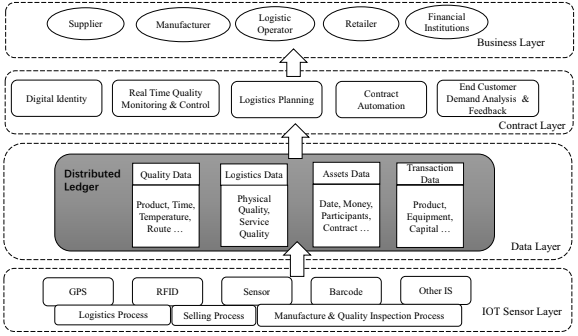
\includegraphics[width=14cm,height=7cm]{supply_chain.png}
    \caption{Supply chain management architecture diagram}
    \label{fig:my_label}
\end{figure}
\subsection{VeChain}
\par VeChain, a startup focusing on supply chain management, has been deploying blockchain technology to record the detailed history of products in order to provide a quick and easy way for consumers and relevant parties to verify their authenticity.
\section{Legal Metrology}
\par Legal metrology is the application of legal requirements to measurements and measuring instruments. Legal metrology embraces the regulation and control of mea-
suring instruments (MI) used in a diversity of applications
including industry, transportation, commerce, medical care
and environment protection.Measurements are so much a part of our daily lives that we often take them for granted and possibly don’t even notice them. For example we monitor the speed at which we drive to ensure we travel safely and thus reduce road casualties, we undergo medical checks to make sure we remain healthy, we consume electricity, gas and water which are billed based on measurements, we have our vehicles checked to monitor the exhaust emission levels
\par The commonality of all of these applications is
that the person executing or being affected by an official
measurement cannot check the determined result; the parties
concerned must rather rely on the accuracy of the measure-
ment. Hence, the central concern of legal metrology is to
protect and ensure that trust, which can also be realized by
blockchain technology.
\section{Internet of Things}
\begin{figure}
    \centering
    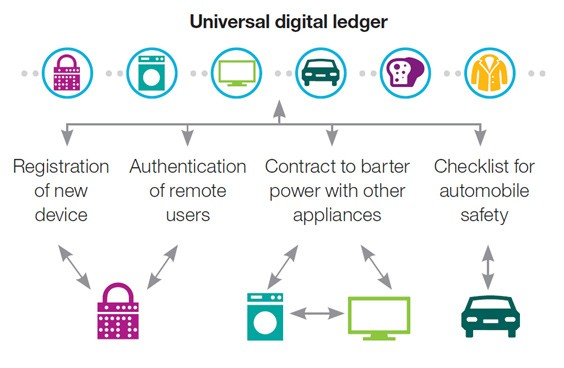
\includegraphics[width=.5\textwidth]{iot.jpg}
    \caption{Blockchain as a distributed ledger in IoT}
    \label{fig:my_label}
\end{figure}

\par IoT is creating new opportunities and providing a competitive advantage for businesses in current and new markets. It touches everything—not just the data, but how, when, where and why you collect it. The technologies that have created the Internet of Things aren’t changing the internet only, but rather change the things connected to the internet—the devices and gateways on the edge of the network that are now able to request a service or start an action without human intervention at many levels.

%1. What have you learned from the existing solutions\\
%2. What were the key points in selecting your work\\
%3. What were the drawbacks you spotted in the existing literature\\




\chapter{Conclusion}
\addcontentsline{toc}{chapter}{Bibliography}

\begin{thebibliography}{100} 

\bibitem{1} Shaohong Fang, Chuanbo Chen, Yunping Zheng, \textquotedblleft An improved colour image representation method by using direct non-symmetery and ant-packing model with triangles and rectangles\textquotedblright, \textit{International Joint Conference on Artificial Intelligence}, 2009.


\bibitem{31} \textquotedblleft Octave-Forge\textquotedblright[Online]\\ 
\textit{Available: http://octave.sourceforge.net/image/function/regionprops.html}


\vspace{2cm}

\textbf{Follow the above format to specify all your references}

\end{thebibliography}

\begin{appendices}
\textbf{The appendix should include your presentation materials (presentation slides), viva questions with the answers that were asked during your presentation and the first page of your reference papers.}
\chapter*{Presentation Slides}
\textbf{It should contain all your presentation slide. Maximum 6 slides per page}
\chapter*{Viva }
\chapter*{References}
\textbf{First page of your reference papers}

\end{appendices}
\end{document}
